%*** SUBSECTION "Module d'estimation des pertes" ***
\subsection{Module 3 : levée d'une alerte}\label{module3}

Pour la levée d'une alerte, nous avons décidé de comparer 3 modèles : 1) un modèle de dérive des concepts via l'estimation classique des pertes  en \textit{concept drift} (voir  section  \ref{pertes}); 2) un modèle par comparaison de courbe ROC (voir  section \ref{roc}); 3)  un modèle basé sur des règles expertes telles que fournies par l'association partenaire (voir  section  \ref{regles}).

\subsubsection{Modèle basé sur l'estimation des pertes}\label{pertes}

La plupart des algorithmes de \emph{concept drift} \cite{Gama2014} considèrent des tâches pour lesquelles on connait, à un certain moment, la vraie valeur associée aux données à prédire. Par exemple, pour des relevés de températures, on peut prédire des valeurs puis mesurer la vraie valeur que l'on peut comparer aux prévisions pour estimer les pertes, c'est-à-dire l'écart entre la prédiction et la vérité et lever une alerte si les pertes sont trop élevées (i.e les prédictions sont trop souvent fausses). Dans notre cas, la "vérité" n'est pas disponible sans intervention du professionnel de santé que l'on souhaite minimiser. Nous avons donc adapté le calcul réalisé par \cite{Bach2010} pour estimer les pertes à un instant donné en considérant le taux d'accord entre les classifieurs (i.e on compte le nombre de classifieurs ayant réalisé la même prédiction).

Soit une fenêtre $\mathcal{F}$ glissante contenant les $N$ derniers exemples de l'utilisateur (lors de l'arrivée d'un nouveau message, le plus ancien est supprimé). Le $1^{er}$ et le $N^e$ exemples décrivent respectivement le message le plus ancien et le plus récent.
Le taux d'erreur $\delta$ au temps $t$, noté $\delta_t$ est donné par :
\[
\delta_t = \frac{\sum\limits_{i=1}^N bienClasse(i)}{N}
\]

où $bienClasse(i)$ retourne le taux d'accord de la prédiction retenue (i.e le nombre de classifieurs ayant prédit le niveau retenu sur le nombre de classifieurs). 

Cependant, il est important de pondérer l'instant dans le temps d'une erreur de classement. Pour cela, un système d'\emph{oubli progressif} (\cite{Chandramouli}) est mis en place. Ainsi, chaque erreur est coefficientée selon son ancienneté :
\[
\delta_t = \frac{\sum\limits_{i=1}^N (bienClasse(i)*\frac{i}{N})}{\frac{N+1}{2}}
\]

Les $N$ dernières valeurs $\delta$ sont mémorisées, soit le $\delta$ associé à chacun des $N$ messages précédemment nommés. 
Une alerte est levée si la moyenne des $N$ $\delta$ dépasse un seuil $\Delta$ fixé par l'utilisateur. Si c'est le cas, l'ensemble des $N$ valeurs $\delta$ sont transmises au module de détection de changement pour calculer le temps pour lequel le changement a eu lieu et lancer une procédure d'alerte auprès du psychiatre référent. 

Pour l'interprétation du professionnel de santé, il est important de lui pointer le temps où un concept est apparu pour l'aider dans son analyse.
Si une dérive du modèle est constatée, il faut réapprendre un nouveau modèle à partir de ce moment. Pour cela, on cherche $\Omega$ tel que :
\begin{itemize} 
\item $\Omega$ soit l'indice de l'exemple parmi l'ensemble des $N$ exemples. Soit $1 \leq \Omega \leq N$;
\item La différence des moyennes des valeurs d'estimation des pertes des sous-ensembles définit par les bornes $[1,\Omega-1]$ et $[\Omega,N]$ soit maximale.
\end{itemize}

Ainsi, l'algorithme~\ref{algo:cd}, que nous proposons, donne le temps $t$ où le changement de concept est le plus plausible. Afin de déterminer au mieux l'instant du changement de comportement.

\begin{algorithm}
\DontPrintSemicolon
\Donnees{Une fenêtre glissante $\mathcal{F}=\{\delta_1, \delta_2, \ldots, \delta_N\}$ de valeurs numériques}
\Res{L'indice $\Omega$ qui maximise l'écart de moyenne entre les sous-ensembles $\mathcal{F}_1$ et $\mathcal{F}_2$ bornés respectivement par $[1,\Omega-1]$ et $[\Omega,N]$}
$\Omega \gets 1$\;
$diff_\Omega \gets 0$\;
\Pour{$i \gets 2$ \textbf{à} $N$} {
	$somme_1 \gets 0$\;
	\Pour{$j \gets 1$ \textbf{à} $i-1$} {
    	$somme_1 = somme_1+ \mathcal{F}_{j}$\;
    }
    $moyenne_1 \gets \frac{somme_1}{i-1}$\;
    
    $somme_2 \gets 0$\;
	\Pour{$j \gets i$ \textbf{à} $N$} {
    	$somme_2 = somme_2+ \mathcal{F}_{j}$\;
    }
    $moyenne_2 \gets \frac{somme_2}{(N-i)+1}$\;
  \Si{$diff_\Omega < |moyenne_1-moyenne_2|$} {
    $\Omega = i$\;
    $diff_\Omega = |moyenne_1-moyenne_2|$\;
  }
}
\Retour{$\Omega$}\;
\caption{{\bsc{Detection du temps de Changement}}}
\label{algo:cd}
\end{algorithm}
\subsubsection{Modèle basé sur la comparaison de courbe ROC}\label{roc}

% Nous avons ici reformuler le problème pour lever une alerte quand on trouve au moins un message posté par l'utilisateur  tel que le niveau de risque associé à ce message soit élevé. Pour atteindre cet objectif, plusieurs approches peuvent être mise en \oe uvre : apprentissage de classifieurs pour le niveau de risque (classification), apprentissage d'une fonction permettant d'associer un risque à chaque message (régression) ou encore apprentissage d'une fonction permettant d'ordonner les messages par risque croissant.

% L'approche que nous allons présenter ici relève de ce dernier cas d'utilisation.
% Nous allons utiliser l'algorithme ROGER (ROc based Genetic learnER) initialement proposé en 2003 dans le cadre de la prédiction du risque cardio-vasculaire \cite{SebagAzeLucas:ICDM2003,SebagLucasAze:EA2003,Challenge_PKDD03}.
% Cet algorithme a été adapté et utilisé avec succès dans plusieurs autres cadres applicatifs : l'extraction de la terminologie \cite{Aze_ROCML:2005}, de la prédiction d'interactions entre protéines \cite{deVienne-Aze_PLoSOne:2012} ou encore de la prédiction de complexes protéines-protéines \cite{PLoSOne:2011}.

% L'algorithme ROGER apprend des fonctions de la forme : $f({\bm x_i}) = \sum_j w_j \times {\bm x_i}(j)$ où ${\bm x_i}(j)$ représente la valeur de la  $j^{ème}$ composante de l'exemple ${\bm x_i}$.
% L'algorithme apprend les poids $w_j$ tels que $\sum_i rang_f({\bm x_i}) \times \mathds{1}_{y_i = +1}$ soit minimale (où $rang_f({\bm x_i})$ correspond au rang de l'exemple ${\bm x_i}$ induit par la fonction $f$, et $\mathds{1}_{y_i = +1}$ correspondant à la fonction indicatrice qui vaut 1 si la classe de ${\bm x_i}$ est positive et 0 sinon).

% Il est aisé de montrer qu'une fonction maximisant l'aire sous la courbe ROC minimise la somme des rangs des exemples positifs qu'elle ordonne.

La  \textbf{courbe ROC} (Receiver Operating Characteristic) \cite{RocLift:2006,ROC:1978} représente un classifieur ayant la capacité de séparer parfaitement les positifs des négatifs.

Nous allons utiliser l'algorithme ROGER (ROc based Genetic learnER) initialement proposé en 2003 dans le cadre de la prédiction du risque cardio-vasculaire \cite{SebagAzeLucas:ICDM2003,SebagLucasAze:EA2003,Challenge_PKDD03}. Cet algorithme a été adapté et utilisé avec succès dans plusieurs autres cadres applicatifs : l'extraction de la terminologie \cite{Aze_ROCML:2005}, de la prédiction d'interactions entre protéines \cite{deVienne-Aze_PLoSOne:2012} ou encore de la prédiction de complexes protéines-protéines \cite{PLoSOne:2011}.

L'algorithme ROGER apprend des fonctions de la forme : $f({\bm x_i}) = \sum_j w_j \times {\bm x_i}(j)$ où ${\bm x_i}(j)$ représente la valeur de la  $j^{ème}$ composante de l'exemple ${\bm x_i}$.
L'algorithme apprend les poids $w_j$ tels que $\sum_i rang_f({\bm x_i}) \times \mathds{1}_{y_i = +1}$ soit minimale (où $rang_f({\bm x_i})$ correspond au rang de l'exemple ${\bm x_i}$ induit par la fonction $f$, et $\mathds{1}_{y_i = +1}$ correspondant à la fonction indicatrice qui vaut 1 si la classe de ${\bm x_i}$ est positive et 0 sinon).


Dans notre contexte, ROGER permet d'apprendre à ordonner les messages des utilisateurs par risque décroissant.
Sous l'hypothèse qu'il existe au moins un \textit{concept drift} par utilisateur, nous considérons que le message le plus à risque (prédit par ROGER) est le message correspondant au drift.
\subsubsection{Modèle basé sur les règles expertes}\label{regles}

%La troisième couche consiste à classer l'instance en deux classes (\textit{alerte} et \textit{non alerte}) selon des règles expertes.  
%Comme il n'est pas possible de compter en permanence sur la participation du professionnel pour étiquer les messages et calculer l'estimation des pertes, 
Nous avons également implémenté des règles expertes fournies par l'association \textit{OADI} pour la levée de l'alerte et nous avons exploré les scénarios suivants. Une alerte est levée si il y a : 
1) un message avec un risque  de niveau 4 dans les $N$ derniers messages;
2)  une augmentation du niveau de risque entre 2 temps consécutifs;
3)  une augmentation du niveau de risque avec un écart de au moins 2 niveaux sur une fenêtre de $N$ messages; Nous ferons varier $N$ pour évaluer les performances pour détecter des changements abrupts ou lents;
4)  des oscillations du niveau de risque.

On obtient alors les règles suivantes : Soit $M$ l'ensemble des $N$ derniers messages d'un utilisateur où $M_1$ correspond au message le plus ancien et $M_N$ au plus récent. On notera $R_i$ le niveau de risque du message $i$.

% * <jeromeaze@gmail.com> 2015-09-21T10:03:18.541Z:
%
%  Dans le contexte, je ne comprend pas 
%
\begin{itemize}
\item  $\exists i, 0\leq i \leq N | R_i = 4$
\item  $\exists i, 0\leq i \leq N-1 | R_i < R_{i+1}$
\item  $\exists i, 0\leq i \leq N-1 | R_i < (R_{i+1}-1)$
\item  $\exists i \exists j, 0\leq i \leq N-1, 0\leq j \leq N-1 | R_i < R_{i+1}, R_j > (R_{j+1})$
\end{itemize}

\begin{figure}[!h]
   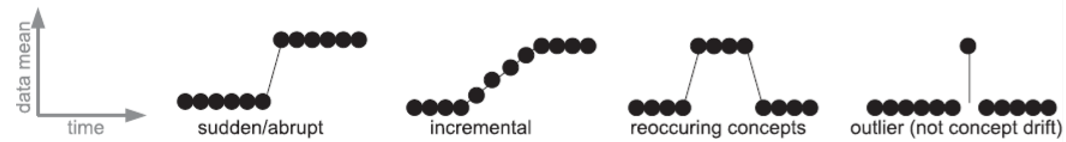
\includegraphics[width=.95\textwidth]{imgs/types_concept_drift.png}
	\caption{\label{formes_cd} Les différentes formes de \emph{concept drift} (adaptés de \cite{Gama2014})}
\end{figure}

Le schéma \ref{formes_cd} représente les différentes formes de changement que nous souhaitons capturer via les règles expertes : 
1) Le changement \emph{immédiat} correspond à un individu qui parle du jour au lendemain de méthode de suicide;
2) Le changement \emph{incrémental} correspond au cas où l'individu parle de plus en plus de son mal être;
3) Le changement \emph{récurrent} est un utilisateur qui régulièrement parle de son mal être;
4) Le \emph{bruit} serait un message isolé parlant de suicide.

%En sortie de ce module, quelque soit les variantes implémentées, nous obtenons la levée ou non d'une alerte pour un individus, le message ayant sucité la levée de l'alerte, les annotations en terme de concept et de risque (issue du module 2) qui vont aider le professionnel de santé à prendre la décision d'intervenir ou non.